\documentclass[hyperref={pdfpagelabels=true}]{beamer}

\usepackage{lmodern}
\usepackage{hyperref}

\title{IESIM: Simulating communities with a game-like approach}   
\subtitle{pecha kucha "style" presentation}
\author{Joana Sim\~{o}es} 
\date{\today} 
\titlegraphic{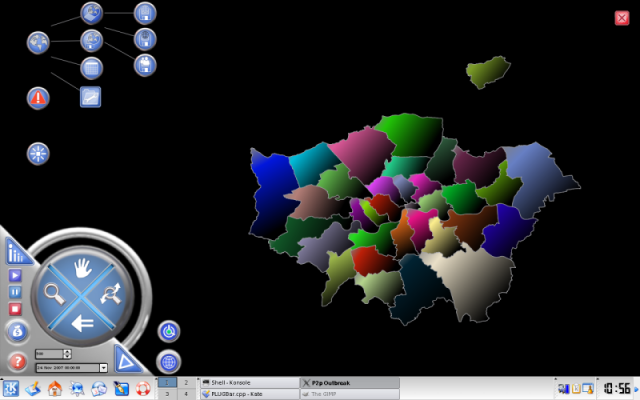
\includegraphics[width=.45\textwidth,height=.35\textheight]{linuxScreen.png}}
 
\usepackage{beamerthemeshadow}
%\usepackage{beamerthemesplit}
\usepackage{listings}

\newcommand{\soooo}{H$_2$SO$_4$}

%fdl stuff
\usepackage{hyperref}
\hypersetup{colorlinks, 
           citecolor=black,
           filecolor=black,
           linkcolor=black,
           urlcolor=black,
           bookmarksopen=true,
           pdftex}

\hfuzz = .6pt % avoid black boxes


\begin{document}
\setbeamertemplate{footline}[page number]
\setbeamertemplate{navigation symbols}{}
\begin{frame}
\transduration{20}
\titlepage
\end{frame} 
 
%\section{Introduction} 
\begin{frame}
\transduration{20}
\frametitle{Introduction}
\begin{overprint}
Which project?
%I worked in many projects, so I decided to choose for this presentation the one I had most fun!
\begin{figure}
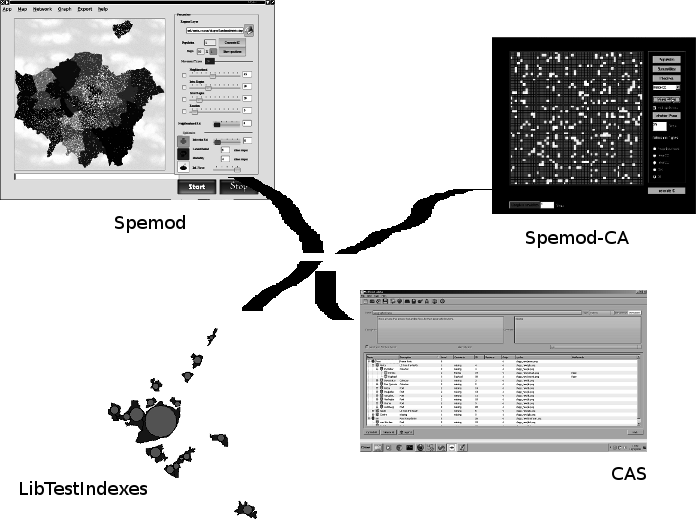
\includegraphics[width=0.5\textwidth]{projects2.png}
\end{figure}
%\pause
    \begin{figure}
    
\includegraphics[scale=0.15]{initial_screen.png}
    \end{figure}
\end{overprint}
\end{frame}

\begin{frame}
\transduration{20}
\frametitle{IeSIM}
%What is the idea behind IeSIM?
IeSIM ADL:
\begin{itemize}
\item Modelling Environment, that implements models through a set of plugins.
\item Targets: programmers and users.
\item Intuitive and easy to use, as a computer game!
\item Cope with lack of data, creating fictitious scenarios (as in games!)
\end{itemize}
%\pause
%To demonstrate better its potentialities we implemented a case study.
\end{frame}

%\section{outbreakP2P} 
\begin{frame}
\transduration{20}
\frametitle{outbreakP2P}
Case Study: outbreakP2P:
\begin{itemize}
%\item Package built using Iesim ADL.
\item Simulates the spreading of a non-vector infectious disease.
\item Split into three sub-models: community, hazard and intervention.
\item Each sub-model is implemented in a separate plugin (ICom, IHaz and IInt).
\end{itemize}
\end{frame}

\begin{frame}
\transduration{20}
\frametitle{Plugins}
Each plugin is loaded at run-time and appears as an icon, which gives access to a set of sub-menus to configure the different model parameters.

\begin{columns}
  \begin{column}{5cm}
    \begin{figure}
    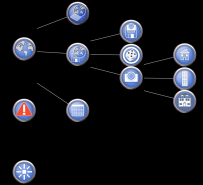
\includegraphics[scale=0.4]{icons.png}
    \end{figure}
  \end{column}
  \begin{column}{5cm}
    \begin{figure}
    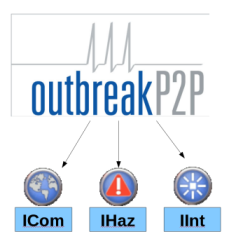
\includegraphics[scale=0.8]{plugins3.png}
    \end{figure}
  \end{column}  
\end{columns}

%So what are the models behind each plugin?
%Bottom up model: Mixed Agent-based/Network approach.
\end{frame}

%\subsection{Community}
\begin{frame}
\transduration{20}
\frametitle{Community}
\begin{itemize}
\item Agents and \textit{Exposure} or \textit{Mixing environments} (ME).
\item Agents: households.
\item ME: functional networks that link the households together. 
\end{itemize}
\begin{figure}
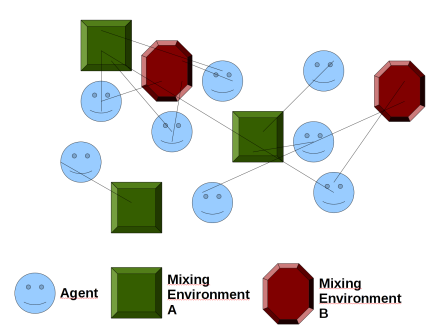
\includegraphics[scale=0.3]{me2.png}
\end{figure}
%\pause
During the configuration, the user loads/generates this information and aggregates the households around the ME.
%Let us see how it works.
\end{frame}

%HOW TO CREATE A COMMUNITY?
\begin{frame}
\transduration{20}
\frametitle{Creating a Community}
\begin{itemize}
\item Step 1: Load population data (e.g.: from a Shapefile)
\begin{figure}
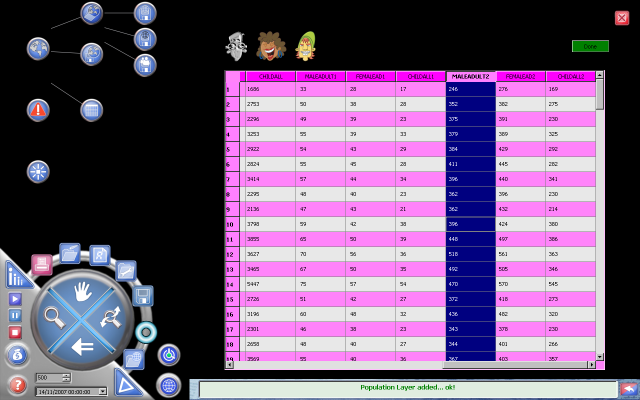
\includegraphics[scale=0.4]{load_population.png}
\end{figure}
\end{itemize}
\end{frame}

\begin{frame}
\transduration{20}
\frametitle{Creating a Community (+)}
\begin{itemize}
\item Step 2: Define the households "structure" (Pert distribution).
\begin{figure}
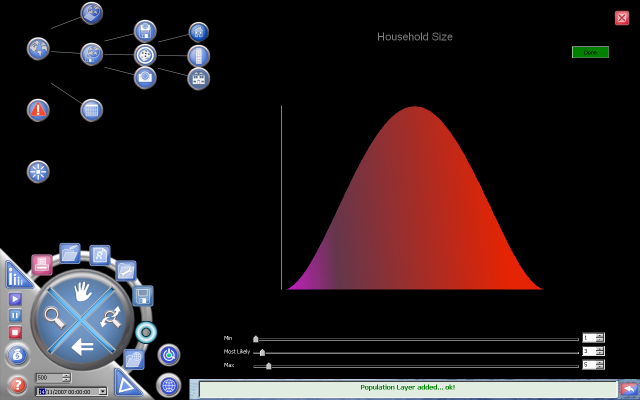
\includegraphics[scale=0.4]{generate_households1.png}
\end{figure}
\end{itemize}
\end{frame}

\begin{frame}
\transduration{20}
\frametitle{Creating a Community (+)}
\begin{itemize}
\item Step 3: Create ME (load them, generate them randomly or input them in the map).
%A buffer is used, to aggregate the households around the ME.
\begin{figure}
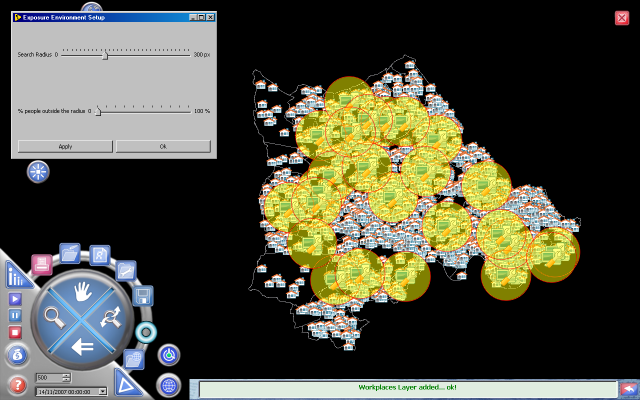
\includegraphics[scale=0.4]{generate_workplaces1.png}
\end{figure}
\end{itemize}
\end{frame}

\begin{frame}
\transduration{20}
\frametitle{Creating a Community (+)}
\begin{itemize}
\item Step 4: Setting the time dynamics of the ME.
%Calendar control: a user friendly UI for a complex task.
\begin{figure}
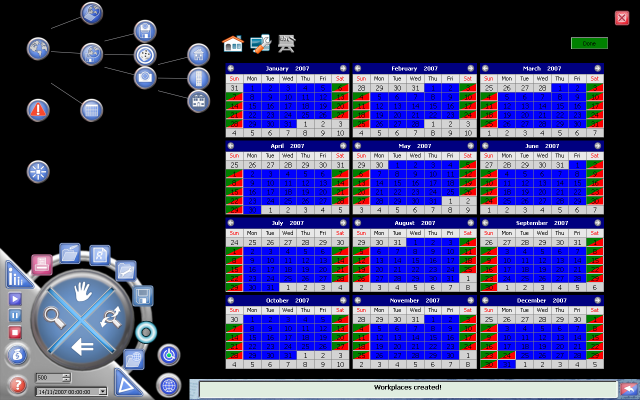
\includegraphics[scale=0.4]{community_dynamics.png}
\end{figure}
\end{itemize}
\end{frame}

%\subsection{Hazard}
\begin{frame}
\transduration{20}
\frametitle{Hazard}
\begin{itemize}
\item Hazard: infectious disease.
\item SEIR model: susceptible, latent, infectious and Removed. %latent period (symptomatic and asymptomatic stages)
\begin{figure}
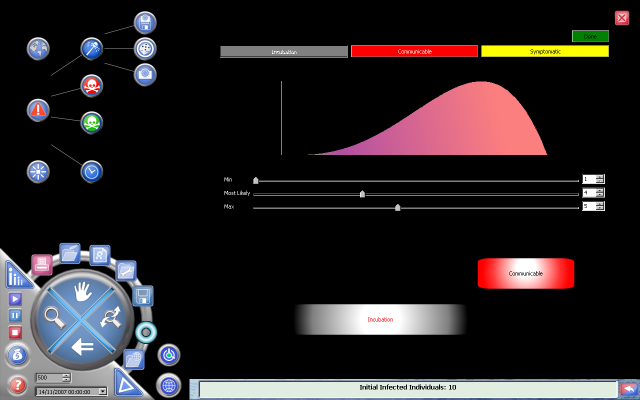
\includegraphics[scale=0.4]{hazard_dynamics.png}
\end{figure}
\end{itemize}
\end{frame}

%\subsection{Hazard}
\begin{frame}
\transduration{20}
\frametitle{Hazard}
\begin{itemize}
\item Set Attack rate ($\beta$) and Illness/Impact rate. %(Pert Distribution).
\item Locate the source of the hazard: known locations of infected individuals.
%Load, generate or input.
\begin{figure}
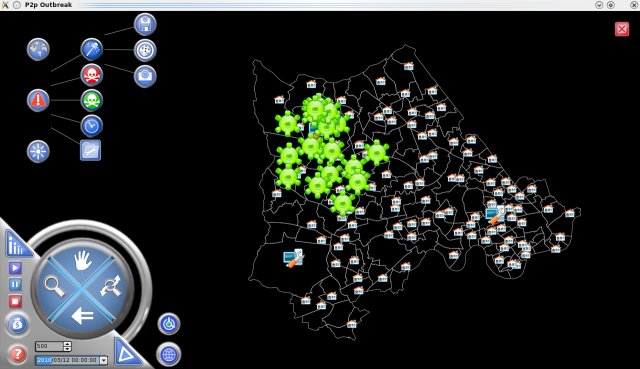
\includegraphics[scale=0.4]{hazard.png}
\end{figure}
\end{itemize}
\end{frame}

%\subsection{Intervention}
\begin{frame}
\transduration{20}
\frametitle{Intervention}
\begin{itemize}
\item Test strategies for the optimal control of an infection in a spatial complex landscape.
%\item Heterogeneous populations: in space and in structure.
\item Vaccination Strategies: proactive and reactive. %Only reactive vaccination was implemented!
\end{itemize}
\begin{figure}
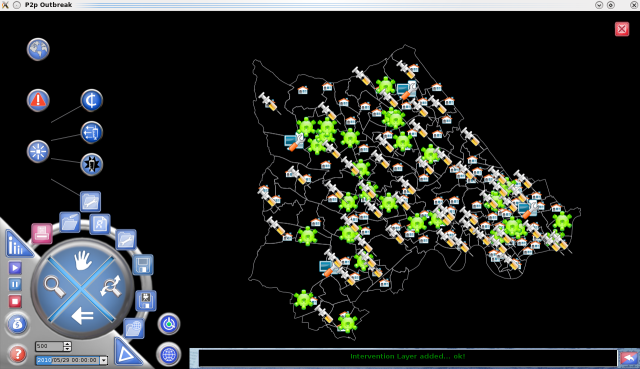
\includegraphics[scale=0.4]{vaccin.png}
\end{figure}
%Configuration procedure similar to the other models
\end{frame}

\begin{frame}
\transduration{20}
\frametitle{Play: Simulate}
\begin{itemize}
\item The simulation integrates information from the three sub-models.
\item Play, stop and pause.
\end{itemize}
\begin{figure}
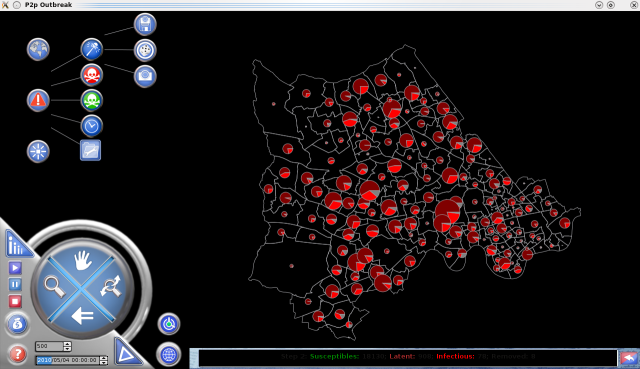
\includegraphics[scale=0.45]{sim.png}
\end{figure}
\end{frame}

\begin{frame}
\transduration{20}
\frametitle{Play: Simulate (+)}
The output of each time step is presented in real time.
\begin{figure}
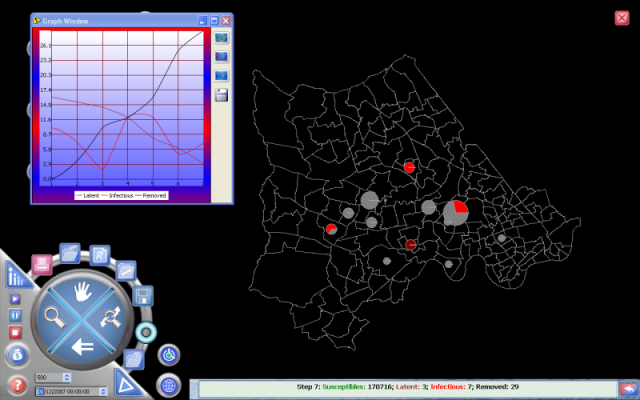
\includegraphics[scale=0.4]{winScreen.png}
\end{figure}
%look at the many elements, including the log window and bar chart
\end{frame}

%\section{Technical Details}
\begin{frame}
\transduration{20}
\frametitle{Some Technical Details}
\begin{itemize}
\item C++ using Qt framework.
\item Native Windows and Linux versions (easily portable to Mac OS).
\item GIS importance: justified the development of an in-house library (GXLib).
\begin{figure}
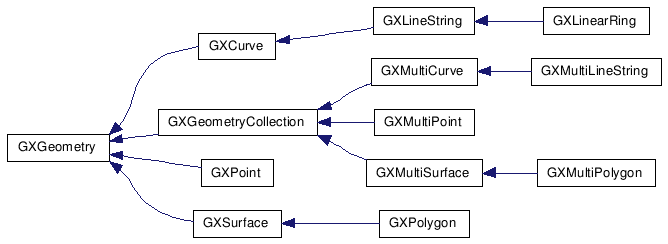
\includegraphics[scale=0.25]{inherit__graph__14.png}
\end{figure}
%Inheritance Diagram of the Geometry class
\end{itemize}
\end{frame}

\begin{frame}
\transduration{20}
\frametitle{Some Technical Details (+)}
\begin{figure}
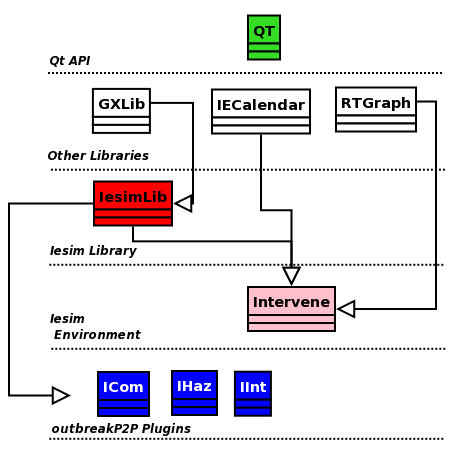
\includegraphics[scale=0.25]{intervene2.png}
\end{figure}
%apart from the GIS library, many cool libraries were developed like the control for setting the time dynamics and the chart
\end{frame}

%\section{Final Remarks}
\begin{frame}
\transduration{20}
\frametitle{Final Remarks}
\begin{itemize}
\item \textit{Game} approach in scientific modelling.
\item Tools to be used by non experts.
\item Product needs a lot of testing, and some features still need to be developed.
\end{itemize}
\end{frame}


\begin{frame}
\transduration{20}
\frametitle{Final Remarks (+)}
\begin{itemize}
\item Unfortunately the end of funding before we could reach a release meant, the "freeze" of the project. %although we won a award in Brazil in a 
%simulation conference (WAMS 2010)
\begin{figure}
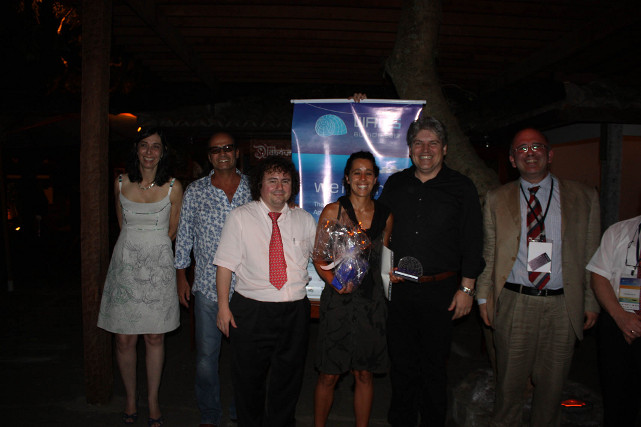
\includegraphics[scale=0.25]{award.jpg}
\end{figure}
\item I am open for collaboration opportunities in the future, that could push IeSIM further.
\end{itemize}
\end{frame}

\begin{frame}
\transduration{20}
\frametitle{Links}
\begin{itemize}
\item IeSim at WAMS 2010: \url{http://tinyurl.com/c7sdeod}
\item Qt project: \url{http://qt-project.org/}
\item \url{http://www.casa.ucl.ac.uk/joanamargarida/}
\item \url{http://www.doublebyte.net}
\end{itemize}
\begin{figure}

\includegraphics[scale=0.4]{thanks.png}
\end{figure}
%and enjoy the rest of the pecha kechua!
\end{frame}

\end{document}

%TODO: check how IESIM is written; test the times; if necessary remove animations; spread some slides; +4 (intervene: 2, one more for the hazard, one more for the intervene

